% ============================================================
%  CHAPITRE : FONCTION LOGARITHME NÉPÉRIEN
%  Mazava Maths — Terminale S
%  Environnements : definition, propriete, theoreme, methode,
%                   attention, astucebac, exemple, exercice,
%                   solution, remarque
% ============================================================

\chapter{Fonction logarithme népérien}

\begin{objectifs}
	\begin{itemize}
		\item Connaître la définition et les propriétés algébriques de $\ln$.
		\item Résoudre des équations, inéquations et systèmes faisant intervenir $\ln$.
		\item Calculer des limites classiques avec $\ln$.
		\item Étudier des fonctions construites à partir de $\ln$.
		\item Calculer des primitives du type $\dfrac{u'}{u}$.
	\end{itemize}
\end{objectifs}

% ----------------------------------------------------------------
\section{Définition et premières propriétés}
% ----------------------------------------------------------------

\begin{definition}
	La fonction \textbf{logarithme népérien}, notée $\ln$, est l'unique
	primitive sur $]0\,;+\infty[$ de la fonction $x \mapsto \dfrac{1}{x}$
	qui s'annule en $x = 1$ :
	\[
	\forall x > 0, \quad (\ln x)' = \frac{1}{x}
	\qquad \text{et} \qquad \ln 1 = 0.
	\]
\end{definition}

\begin{propriete}{Sens de variation et signe}{}
	La fonction $\ln$ est \textbf{strictement croissante} sur $]0\,;+\infty[$
	car $(\ln x)' = \dfrac{1}{x} > 0$ pour tout $x > 0$.
	
	De plus :
	\[
	\ln x < 0 \iff 0 < x < 1, \qquad
	\ln x = 0 \iff x = 1, \qquad
	\ln x > 0 \iff x > 1.
	\]
\end{propriete}

\begin{propriete}{Propriétés algébriques}{}
	Pour tous réels $a > 0$ et $b > 0$, et pour tout $n \in \Z$, $\alpha \in \R$ :
	\begin{center}
		\renewcommand{\arraystretch}{2.0}
		\begin{tabular}{|c|c|}
			\hline
			\textbf{Propriété} & \textbf{Formule} \\
			\hline
			Produit & $\ln(a \cdot b) = \ln a + \ln b$ \\
			\hline
			Quotient & $\ln\!\left(\dfrac{a}{b}\right) = \ln a - \ln b$ \\
			\hline
			Inverse & $\ln\!\left(\dfrac{1}{b}\right) = -\ln b$ \\
			\hline
			Puissance entière & $\ln(a^n) = n\ln a$ \\
			\hline
			Puissance réelle & $\ln(a^\alpha) = \alpha \ln a$ \\
			\hline
			Racine carrée & $\ln\!\left(\sqrt{a}\right) = \dfrac{1}{2}\ln a$ \\
			\hline
		\end{tabular}
	\end{center}
\end{propriete}

\begin{attention}
	$\ln(a + b) \neq \ln a + \ln b$ \quad et \quad
	$\ln(a \times b) \neq \ln a \times \ln b$.
	
	Ces erreurs sont très fréquentes au BAC.
\end{attention}

\begin{exemple}
	Simplifier les expressions suivantes :
	\[
	A = \ln 6 + \ln 3 - \ln 2, \qquad
	B = \ln\sqrt{5} + \ln\sqrt{20}, \qquad
	C = 2\ln 3 - \ln 9.
	\]
	\textbf{Solution :}
	\[
	A = \ln\!\frac{6 \times 3}{2} = \ln 9 = 2\ln 3.
	\]
	\[
	B = \ln\!\left(\sqrt{5} \times \sqrt{20}\right) = \ln\sqrt{100} = \ln 10.
	\]
	\[
	C = \ln 3^2 - \ln 9 = \ln 9 - \ln 9 = 0.
	\]
\end{exemple}

% ----------------------------------------------------------------
\section{Limites usuelles}
% ----------------------------------------------------------------

\begin{propriete}{Limites aux bornes et limites classiques}{}
	\begin{center}
		\renewcommand{\arraystretch}{2.2}
		\begin{tabular}{|c|c|}
			\hline
			\textbf{Limite} & \textbf{Résultat} \\
			\hline
			$\displaystyle\lim_{x \to 0^+} \ln x$ & $-\infty$ \\
			\hline
			$\displaystyle\lim_{x \to +\infty} \ln x$ & $+\infty$ \\
			\hline
			$\displaystyle\lim_{x \to +\infty} \frac{\ln x}{x^n}$ \quad ($n \geq 1$)
			& $0$ \quad (ln négligeable devant $x^n$) \\
			\hline
			$\displaystyle\lim_{x \to 0^+} x^n \ln x$ \quad ($n \geq 1$)
			& $0$ \quad (ln écrasé par $x^n$) \\
			\hline
			$\displaystyle\lim_{x \to 0} \frac{\ln(1+x)}{x}$
			& $1$ \\
			\hline
			$\displaystyle\lim_{x \to 1} \frac{\ln x}{x-1}$
			& $1$ \\
			\hline
		\end{tabular}
	\end{center}
\end{propriete}

\begin{astucebac}
	Les deux dernières limites servent souvent à lever des
	formes indéterminées $\dfrac{0}{0}$ au BAC.
	On les retrouve aussi dans l'étude de la dérivabilité de fonctions en un point.
\end{astucebac}

\begin{exemple}
	Calculer $\displaystyle\lim_{x \to +\infty} \frac{\ln(x^2+1)}{x}$.
	
	On écrit $\ln(x^2+1) = \ln\!\left(x^2\!\left(1+\frac{1}{x^2}\right)\right)
	= 2\ln x + \ln\!\left(1+\frac{1}{x^2}\right)$.
	
	Donc $\dfrac{\ln(x^2+1)}{x} = \dfrac{2\ln x}{x} + \dfrac{\ln(1+1/x^2)}{x}
	\xrightarrow[x\to+\infty]{} 0 + 0 = 0$.
\end{exemple}

% ----------------------------------------------------------------
\section{Dérivée et dérivée de fonctions composées}
% ----------------------------------------------------------------

\begin{propriete}{Dérivées avec $\ln$}{}
	\begin{center}
		\renewcommand{\arraystretch}{2.2}
		\begin{tabular}{|c|c|c|}
			\hline
			\textbf{Fonction} & \textbf{Dérivée} & \textbf{Condition} \\
			\hline
			$\ln x$ & $\dfrac{1}{x}$ & $x > 0$ \\
			\hline
			$\ln u$ & $\dfrac{u'}{u}$ & $u > 0$ \\
			\hline
			$\ln |u|$ & $\dfrac{u'}{u}$ & $u \neq 0$ \\
			\hline
			$\ln(ax+b)$ & $\dfrac{a}{ax+b}$ & $ax+b > 0$ \\
			\hline
		\end{tabular}
	\end{center}
\end{propriete}

\begin{methode}
	Pour dériver $\ln[u(x)]$ :
	\begin{enumerate}
		\item Identifier $u(x)$.
		\item Calculer $u'(x)$.
		\item Appliquer : $\bigl(\ln u\bigr)' = \dfrac{u'}{u}$.
	\end{enumerate}
\end{methode}

\begin{exemple}
	Calculer les dérivées des fonctions suivantes :
	\[
	f(x) = \ln(3x^2+1), \qquad
	g(x) = \ln\!\left(\frac{x+1}{x-1}\right) \text{ sur } ]1\,;+\infty[, \qquad
	h(x) = x\ln x.
	\]
	\[
	f'(x) = \frac{6x}{3x^2+1}.
	\]
	\[
	g(x) = \ln(x+1) - \ln(x-1) \implies
	g'(x) = \frac{1}{x+1} - \frac{1}{x-1} = \frac{-2}{x^2-1}.
	\]
	\[
	h'(x) = \ln x + x \cdot \frac{1}{x} = \ln x + 1.
	\]
\end{exemple}

% ----------------------------------------------------------------
\section{Étude complète de la fonction $\ln$}
% ----------------------------------------------------------------

\begin{propriete}{Tableau de variation de $\ln$}{}
	\begin{center}
		\begin{tikzpicture}
			\tkzTabInit[lgt=3, espcl=4]{
				$x$ / 1,
				$(\ln x)'=\frac{1}{x}$ / 1,
				$\ln x$ / 2
			}{
				$0$, $1$, $+\infty$
			}
			\tkzTabLine{d, +, , +,}
			\tkzTabVar{D- / $-\infty$, R / $0$, +/ $+\infty$}
		\end{tikzpicture}
	\end{center}
\end{propriete}

\begin{remarque}
	Si \texttt{tkz-tab} n'est pas disponible, voici la version texte du tableau :
	
	\medskip
	\begin{center}
		\renewcommand{\arraystretch}{1.6}
		\begin{tabular}{|c|ccccc|}
			\hline
			$x$ & $0$ & & $1$ & & $+\infty$ \\
			\hline
			$(\ln x)'$ & & $+$ & & $+$ & \\
			\hline
			$\ln x$ & $-\infty$ & $\nearrow$ & $0$ & $\nearrow$ & $+\infty$ \\
			\hline
		\end{tabular}
	\end{center}
\end{remarque}

% Figure TikZ — courbe de ln
\begin{center}
	\begin{tikzpicture}[>=Stealth, scale=1.1]
		\draw[->] (-0.3,0) -- (5.5,0) node[right, font=\small] {$x$};
		\draw[->] (0,-2.2) -- (0,2.2) node[above, font=\small] {$y$};
		% graduations
		\foreach \x in {1,2,3,4,5}{
			\draw (\x,2pt)--(\x,-2pt) node[below,font=\tiny]{\x};
		}
		\foreach \y in {-2,-1,1,2}{
			\draw (2pt,\y)--(-2pt,\y) node[left,font=\tiny]{\y};
		}
		% courbe ln
		\draw[thick, domain=0.13:5.2, samples=100]
		plot(\x, {ln(\x)});
		% tangente en x=1 (pente 1)
		\draw[dashed, gray] (-0.3,-1.3)--(2.3,1.3)
		node[right, font=\tiny, gray]{tangente en $x=1$};
		% point (1,0)
		\filldraw (1,0) circle(2pt) node[above right, font=\small]{$(1,0)$};
		% label courbe
		\node[right, font=\small] at (4.5, {ln(4.5)}) {$\mathcal{C}_{\ln}$};
		% origine
		\node[below left, font=\small] at (0,0){$O$};
	\end{tikzpicture}
\end{center}

% ----------------------------------------------------------------
\section{Équations et inéquations avec $\ln$}
% ----------------------------------------------------------------

\begin{methode}
	\textbf{Équations :}
	\begin{itemize}
		\item $\ln[u(x)] = a \iff u(x) = \e^a$ \quad (et $u(x)>0$).
		\item $\ln[u(x)] = \ln[v(x)] \iff u(x) = v(x)$ \quad (et $u,v > 0$).
	\end{itemize}
	\textbf{Inéquations :} $\ln$ est croissante, donc :
	\[
	\ln[u(x)] \leq \ln[v(x)] \iff u(x) \leq v(x) \quad
	\text{(sous réserve que } u,v > 0\text{)}.
	\]
\end{methode}

\begin{exemple}
	Résoudre dans $\R$ :
	\[
	\text{a)}\quad \ln(2x-1) = \ln(x+3)
	\qquad
	\text{b)}\quad \ln(x^2-3) \leq \ln(2x)
	\qquad
	\text{c)}\quad \ln x + \ln(x-2) = \ln 3
	\]
	
	\textbf{a)} $2x-1 = x+3$ et $2x-1>0 \Rightarrow x=4$. \quad $S=\{4\}$.
	
	\textbf{b)} Conditions : $x^2-3>0$ et $2x>0$, soit $x>\sqrt{3}$.
	Sur cet ensemble : $x^2-3 \leq 2x \Rightarrow x^2-2x-3\leq 0
	\Rightarrow (x-3)(x+1)\leq 0 \Rightarrow x\leq 3$.
	Donc $S = ]\sqrt{3}\,;3]$.
	
	\textbf{c)} $\ln[x(x-2)] = \ln 3$, conditions $x>2$ :
	$x^2-2x=3 \Rightarrow x^2-2x-3=0 \Rightarrow x=3$ ou $x=-1$.
	Avec $x>2$ : $S=\{3\}$.
\end{exemple}

% ----------------------------------------------------------------
\section{Primitives avec $\ln$}
% ----------------------------------------------------------------

\begin{propriete}{Primitives faisant intervenir $\ln$}{}
	\begin{center}
		\renewcommand{\arraystretch}{2.2}
		\begin{tabular}{|c|c|c|}
			\hline
			\textbf{Fonction} & \textbf{Primitive} & \textbf{Condition} \\
			\hline
			$\dfrac{1}{x}$ & $\ln|x|$ & $x \neq 0$ \\
			\hline
			$\dfrac{u'}{u}$ & $\ln|u|$ & $u \neq 0$ \\
			\hline
			$\dfrac{u'}{u}$ & $\ln u$ & $u > 0$ \\
			\hline
			$\dfrac{a}{ax+b}$ & $\ln|ax+b|$ & $ax+b \neq 0$ \\
			\hline
		\end{tabular}
	\end{center}
\end{propriete}

\begin{astucebac}
	Dès que vous voyez une fraction dont le \textbf{numérateur est la dérivée
		du dénominateur} (à un coefficient près), pensez immédiatement à $\ln|u|$.
\end{astucebac}

\begin{exemple}
	Calculer les primitives suivantes :
	\[
	\text{a)}\quad \int \frac{2x}{x^2+1}\dd x
	\qquad
	\text{b)}\quad \int \frac{3}{3x-2}\dd x
	\qquad
	\text{c)}\quad \int \frac{x^2+1}{x^3+3x}\dd x
	\]
	\textbf{a)} $u=x^2+1$, $u'=2x$ : primitive $= \ln(x^2+1)+C$.
	
	\textbf{b)} $u=3x-2$, $u'=3$ : primitive $= \ln|3x-2|+C$.
	
	\textbf{c)} $u=x^3+3x$, $u'=3x^2+3=3(x^2+1)$. On écrit :
	$\dfrac{x^2+1}{x^3+3x} = \dfrac{1}{3}\cdot\dfrac{3(x^2+1)}{x^3+3x} = \dfrac{u'}{3u}$.
	Primitive $= \dfrac{1}{3}\ln|x^3+3x|+C$.
\end{exemple}

% ----------------------------------------------------------------
\section{Exercices résolus}
% ----------------------------------------------------------------

\exercice{\etoilepleine\etoilevide\etoilevide}
\begin{enumerate}
	\item Simplifier : $A = \ln 12 - \ln 3 + \ln\!\left(\dfrac{1}{4}\right)$.
	\item Résoudre dans $\R$ : $\ln(x+2) + \ln(x-1) = \ln 4$.
	\item Calculer $f'(x)$ pour $f(x) = \ln(x^2+x+1)$.
\end{enumerate}

\solution

\textbf{1.}
$A = \ln\!\dfrac{12}{3} + \ln\!\dfrac{1}{4}
= \ln 4 + \ln\!\dfrac{1}{4}
= \ln\!\left(4 \times \dfrac{1}{4}\right)
= \ln 1 = 0.$

\textbf{2.} Conditions : $x+2>0$ et $x-1>0$, soit $x>1$.
\[
\ln[(x+2)(x-1)] = \ln 4
\implies (x+2)(x-1) = 4
\implies x^2+x-6 = 0
\implies (x-2)(x+3)=0.
\]
Avec $x>1$ : $\boxed{S = \{2\}}$.

\textbf{3.} $u = x^2+x+1$, $u'=2x+1$ :
\[
f'(x) = \frac{2x+1}{x^2+x+1}.
\]

\bigskip
\exercice{\etoilepleine\etoilepleine\etoilevide}
Soit $f$ la fonction définie sur $]0\,;+\infty[$ par $f(x) = x - 1 - \ln x$.
\begin{enumerate}
	\item Calculer $f'(x)$ et dresser le tableau de variation de $f$.
	\item Démontrer que $\forall x > 0,\; \ln x \leq x - 1$.
	\item En déduire que $\forall x > 0,\; \ln x \leq x - 1$.
	Quelle est l'égalité et en quel point ?
\end{enumerate}

\solution

\textbf{1.}
$f'(x) = 1 - \dfrac{1}{x} = \dfrac{x-1}{x}$.

\begin{center}
	\renewcommand{\arraystretch}{1.6}
	\begin{tabular}{|c|ccccc|}
		\hline
		$x$ & $0$ & & $1$ & & $+\infty$ \\
		\hline
		$f'(x)$ & & $-$ & $0$ & $+$ & \\
		\hline
		$f(x)$ & $+\infty$ & $\searrow$ & $0$ & $\nearrow$ & $+\infty$ \\
		\hline
	\end{tabular}
\end{center}

\textbf{2.} $f$ admet un minimum global en $x=1$ valant $f(1)=0$.
Donc $\forall x>0,\; f(x) \geq 0$, soit $x-1-\ln x \geq 0$,
c'est-à-dire $\ln x \leq x-1$.

\textbf{3.} L'égalité $\ln x = x-1$ a lieu si et seulement si $f(x)=0$,
soit en $x=1$.

\bigskip
\exercice{\etoilepleine\etoilepleine\etoilepleine}
Calculer $\displaystyle I = \int_1^{\e} \frac{\ln x}{x}\dd x$
et $\displaystyle J = \int_1^{\e} \ln x \dd x$.

\solution

\textbf{Calcul de $I$.}
On pose $u = \ln x$, donc $u' = \dfrac{1}{x}$.
On reconnaît $\dfrac{\ln x}{x} = u' \cdot u = u \cdot u'$, donc :
\[
I = \left[\frac{(\ln x)^2}{2}\right]_1^{\e}
= \frac{(\ln \e)^2}{2} - \frac{(\ln 1)^2}{2}
= \frac{1}{2} - 0 = \frac{1}{2}.
\]

\textbf{Calcul de $J$ par IPP.}
On pose $u = \ln x$, $v' = 1$, donc $u' = \dfrac{1}{x}$, $v = x$ :
\[
J = \Big[x\ln x\Big]_1^{\e} - \int_1^{\e} x \cdot \frac{1}{x}\dd x
= \Big[x\ln x\Big]_1^{\e} - \int_1^{\e} 1\dd x
= (\e\ln\e - 1\cdot\ln 1) - [\e - 1]
= \e - 0 - \e + 1 = 1.
\]

% ----------------------------------------------------------------
\section{Exercice type BAC}
% ----------------------------------------------------------------

\exercice{\etoilepleine\etoilepleine\etoilepleine}

\textit{(D'après BAC Série S — Madagascar)}

\medskip
Soit $f$ la fonction définie sur $]0\,;+\infty[$ par :
\[
f(x) = x - 2 + \frac{1}{\ln x}.
\]
On note $\mathcal{C}$ sa courbe représentative dans un repère orthonormé.

\medskip
\textbf{Partie A : Étude de $f$}
\begin{enumerate}
	\item Calculer $\displaystyle\lim_{x\to 0^+} f(x)$ et
	$\displaystyle\lim_{x\to +\infty} f(x)$.
	\item Calculer $f'(x)$ pour tout $x\in]0\,;1[\,\cup\,]1\,;+\infty[$.
	Dresser le tableau de variation de $f$.
	\item Montrer que la droite $\Delta$ d'équation $y = x-2$ est
	asymptote à $\mathcal{C}$ en $+\infty$.
	Étudier la position de $\mathcal{C}$ par rapport à $\Delta$.
\end{enumerate}

\textbf{Partie B : Intégrale}
\begin{enumerate}
	\setcounter{enumi}{3}
	\item Calculer $\displaystyle\int_{\e}^{\e^2} f(x)\dd x$.
\end{enumerate}

\solution

\textbf{1. Limites.}
\[
\lim_{x\to 0^+} \ln x = -\infty \implies
\lim_{x\to 0^+} \frac{1}{\ln x} = 0^-.
\implies \lim_{x\to 0^+} f(x) = 0 - 2 + 0 = -2.
\]
\[
\lim_{x\to+\infty}\frac{1}{\ln x} = 0 \implies
\lim_{x\to+\infty} f(x) = +\infty.
\]

\textbf{2. Dérivée.}
\[
f'(x) = 1 - \frac{1}{x(\ln x)^2}.
\]
On étudie le signe de $f'(x) = \dfrac{x(\ln x)^2 - 1}{x(\ln x)^2}$.

Le dénominateur $x(\ln x)^2 > 0$ sur le domaine.
Le numérateur $x(\ln x)^2 - 1$ : en $x=\e$, vaut $\e \cdot 1 - 1 = \e-1>0$.

Une étude montre qu'il existe $x_0 \in ]0;1[$ tel que $f'(x_0)=0$
(on admet ce résultat et on dresse le tableau avec le minimum).

\begin{center}
	\renewcommand{\arraystretch}{1.6}
	\begin{tabular}{|c|ccccc|}
		\hline
		$x$ & $0$ & & $x_0$ & & $+\infty$ \\
		\hline
		$f'(x)$ & & $-$ & $0$ & $+$ & \\
		\hline
		$f(x)$ & & $\searrow$ & $f(x_0)$ & $\nearrow$ & $+\infty$ \\
		\hline
	\end{tabular}
\end{center}

\textbf{3. Asymptote.}
$f(x) - (x-2) = \dfrac{1}{\ln x} \xrightarrow[x\to+\infty]{} 0$.
Donc $\Delta : y=x-2$ est asymptote oblique à $\mathcal{C}$ en $+\infty$.

Position : $f(x)-(x-2) = \dfrac{1}{\ln x} > 0$ pour $x>1$,
donc $\mathcal{C}$ est \textbf{au-dessus} de $\Delta$ pour $x>1$.

\textbf{4. Intégrale.}
\[
\int_{\e}^{\e^2} f(x)\dd x
= \int_{\e}^{\e^2} \!\left(x - 2 + \frac{1}{\ln x}\right)\dd x.
\]
\[
= \left[\frac{x^2}{2} - 2x\right]_{\e}^{\e^2}
+ \int_{\e}^{\e^2}\frac{1}{\ln x}\dd x.
\]
Pour $\displaystyle\int_{\e}^{\e^2}\frac{1}{\ln x}\dd x$,
on effectue le changement de variable $t = \ln x$
($\dd x = \e^t \dd t$, bornes $1$ et $2$) :
\[
\int_1^2 \frac{\e^t}{t}\dd t.
\]
Cette intégrale n'a pas de forme close élémentaire — dans un sujet BAC,
elle est en général donnée ou évaluée numériquement.

Pour la partie polynomiale :
\[
\left[\frac{x^2}{2}-2x\right]_{\e}^{\e^2}
= \left(\frac{\e^4}{2}-2\e^2\right) - \left(\frac{\e^2}{2}-2\e\right)
= \frac{\e^4-3\e^2}{2} + 2\e.
\]